\chapter{Behaviour analysis of antennas}
In this Chapter we analyse and discuss each antenna behaviour looking at the results obtained in predicting the gain solutions from each experiment of our learning algorithms for both polarization H in Section \ref{Hp} and V polarization in Section \ref{Vp}. 

\section{Pointing sensor distribution}
\begin{figure}[H]
    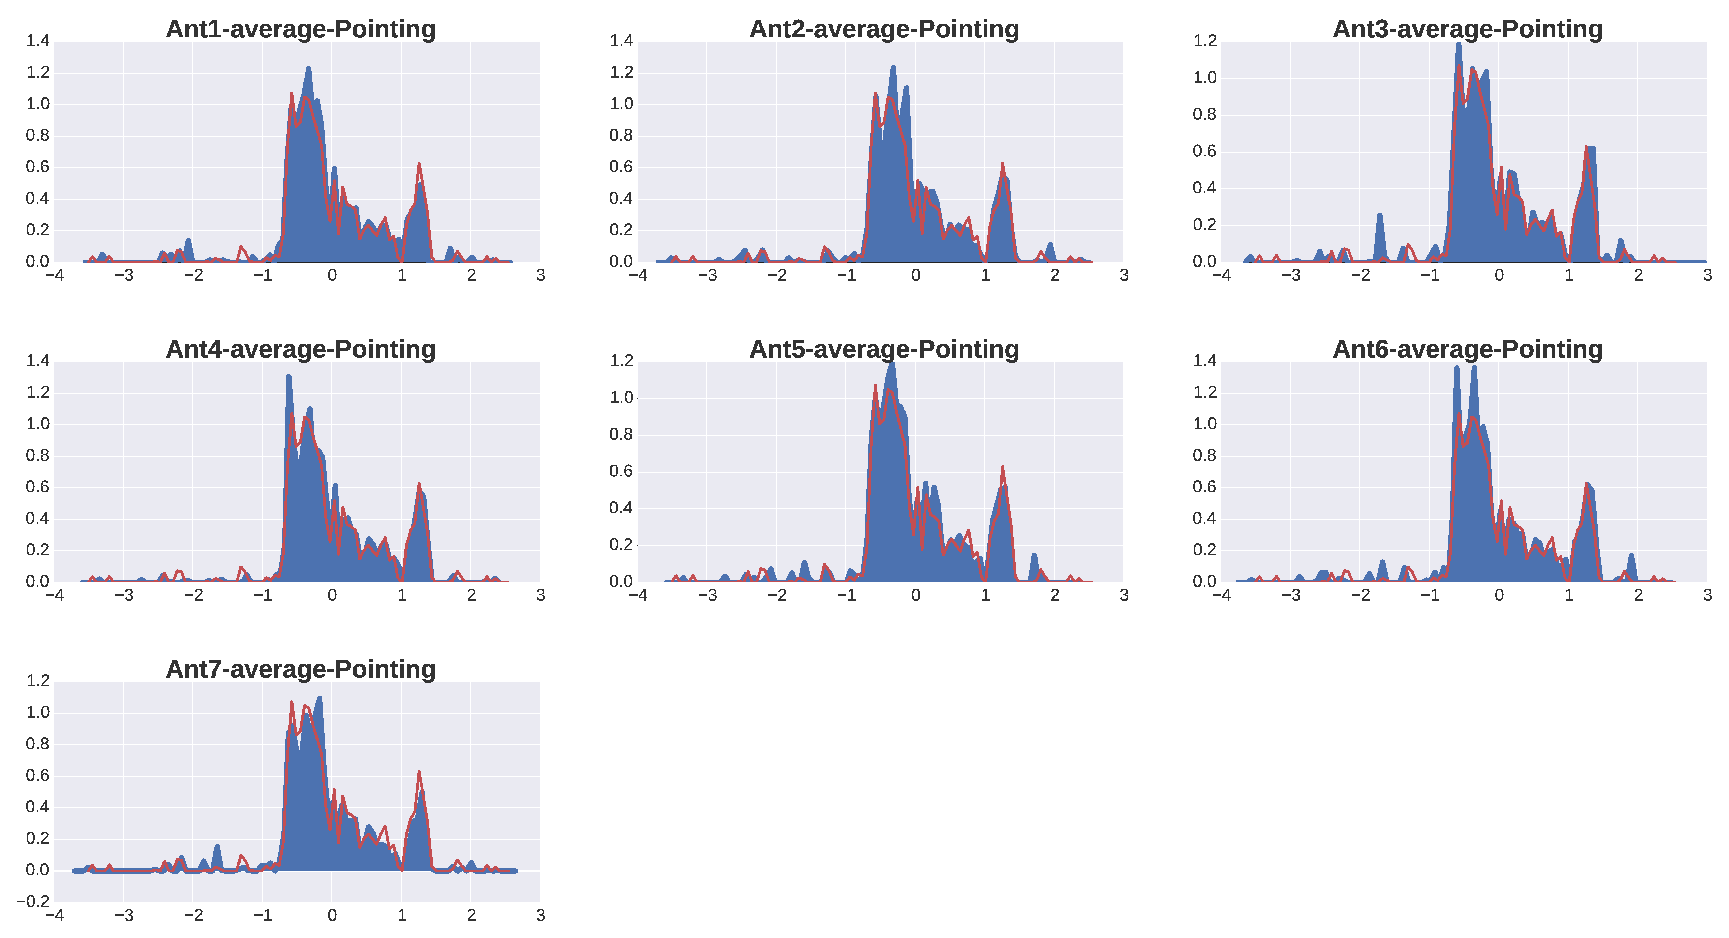
\includegraphics[ height=12cm, width=16cm]{images/Distribution.eps}
    \caption{This figure is showing the distribution of the averaged pointing data per antenna during the tracking of the calibrator source PKS1613-586. The blue line is the average pointing per antenna, and the red line is the reference probability distribution for all the antennas.}
    \label{Point}
\end{figure}
The Figure \ref{Point} illustrate how the pointing sensor data per antenna are distributed. This gives us details about whether or not the antennas were pointing at the same position. We observe that Each antenna pointing is distributed differently from the reference probability distribution. These small offsets might have contribution in prediction errors of amplitude and phase gain solutions.

\section{H-polarization amplitude and phase}
\label{Hp}
As seen in Figure \ref{phase}, the gain phase solutions obtained from CASA for antenna 5 is zero. This is due to the selection of antenna 5 as a reference antenna during the calibration of G solutions. Fundamentally, the baseline visibility phases measured by an interferometry are exclusively different between antennas, and so no absolute phase reference exists \citep{taylor1999synthesis}. Antenna-based calibration solutions thus have phases which are constrained only to satisfy the observed visibility phases; further, each solution in time is formally independent of all others \citep{taylor1999synthesis}, though stability (or at least continuity) in time is expected. Therefore, to assert phase continuity in time, it is conventional practice to assign a reference antenna whose phase will be held constant at zero in time. Also, it is best to choose a reference antenna that never drops out \citep{editioncasa}. 

\begin{figure}[H]
  \centering
    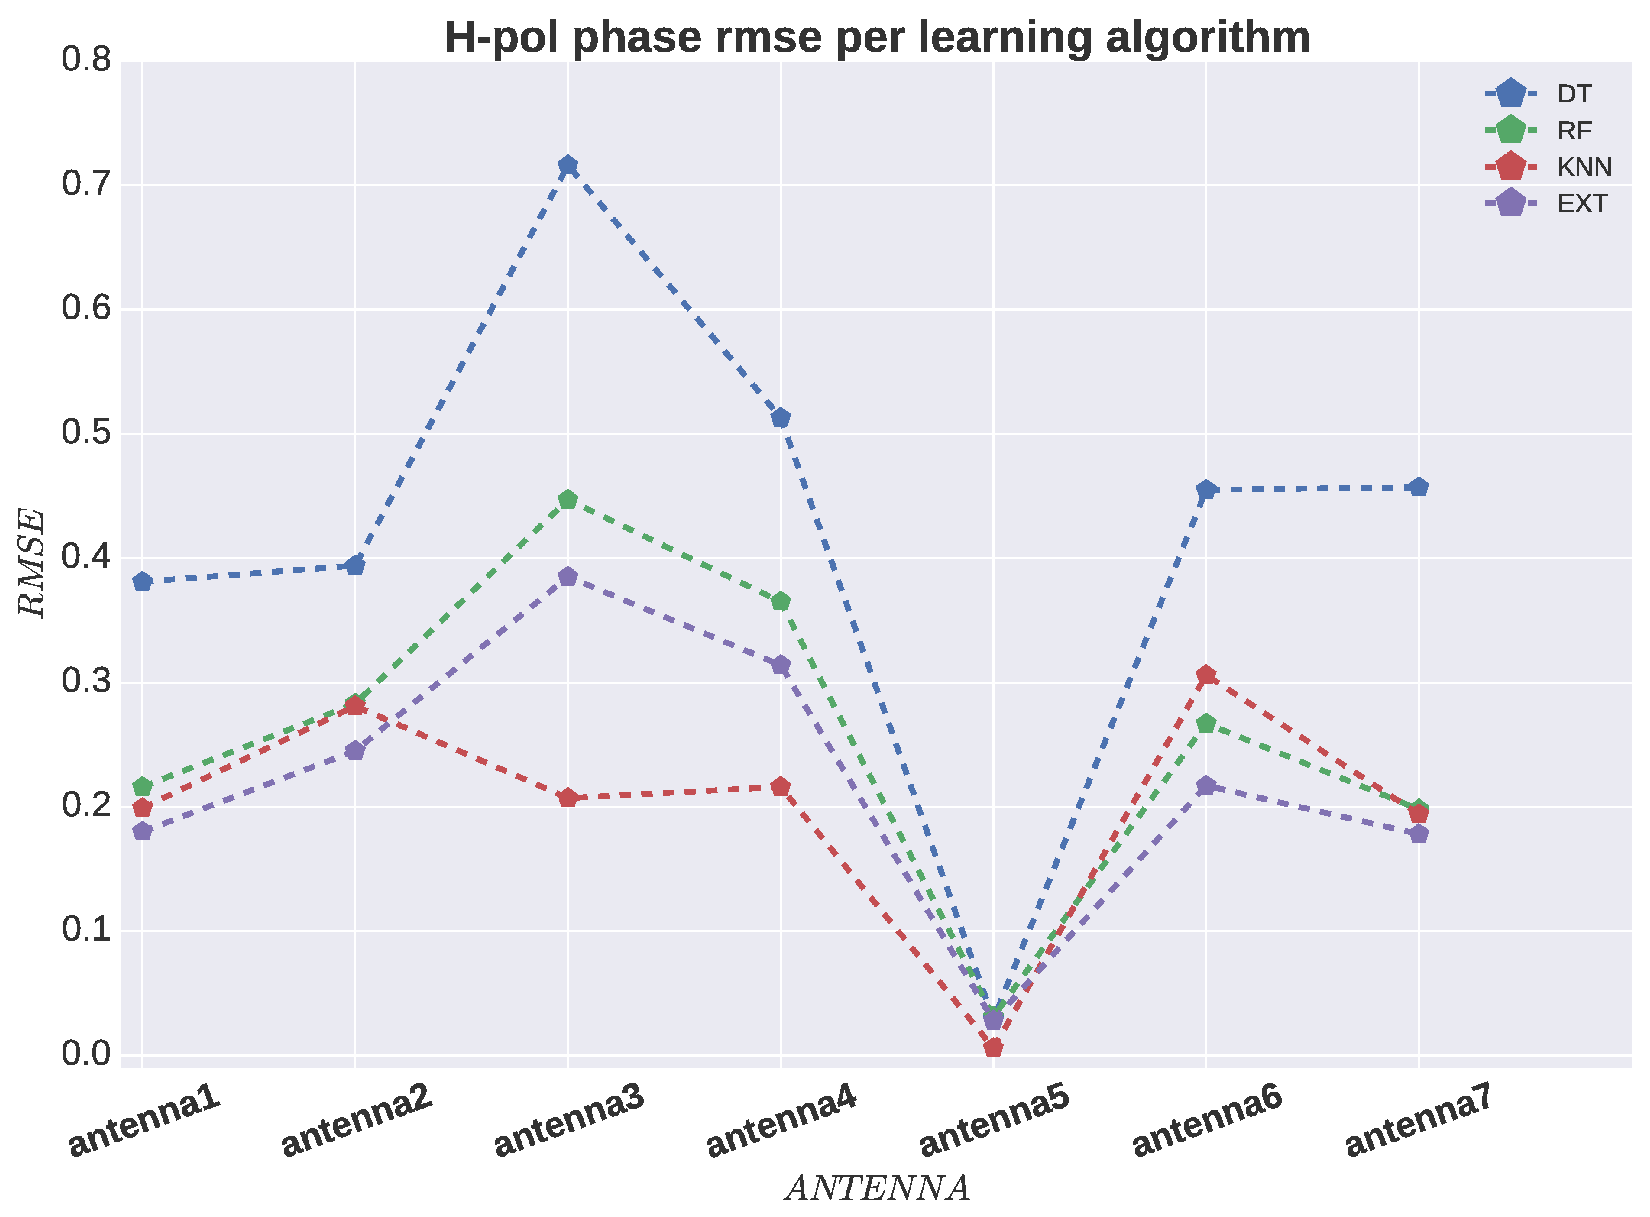
\includegraphics[width=0.6\textwidth]{images/Hpol-phase.eps}
    \caption{Root mean square error for each learning algorithm in predicting the h polarization phase gain solutions for each antenna. The blue, green, red and purple lines represent the different learning algorithms used in our experiment.}
  \label{phrm}
 \end{figure}
From our experiment in Section \ref{sec3} and Figure \ref{phrm}, we observe that the learning algorithms have learned this behaviour pattern with rms error accuracy $\approx$ 0, resulting in predicting zero phase gain solutions for antenna 5. We validated our models looking at 3 observational validation data sets namely: observation test-1,test-2 and test-3. We provide our models with sensor data during tracking of the calibrator source PKS1613-586 as input. The phase output predictions in Figures \ref{obs1}, \ref{obs2}, \ref{obs3}, \ref{obs3}, \ref{obs5}, \ref{obs6}, \ref{obs7}, \ref{obs8}, \ref{obs9}, \ref{obs10}, \ref{obs11}, \ref{obs12}  certainly prove that the models have learned to generalize for the reference antenna, by predicting zero phases for antenna 5 h and v polarization as trained, assuming that the antenna was stable without any drop-outs during the period of the observation. In Figure \ref{phrm}, Though the models suppose to perform differently due to their parameter settings, we notice that the random forest, K-nearest neighbor and the extremely randomised trees methods are very close to each other in rms error as function of antenna 1h, 2h, 5h, 6h and 7h, whereas there is large variation in rms error for antenna 3h and 4h. With such behaviour, this gives us an idea about the instability of these two antennas. Figure \ref{phrm} also illustrate which model can be used for better predictions of h polarization phase gain solutions. In this case, we observe that the decision tree model is having large rms error scatter than the random forest, K-nearest neighbors and the extremely randomized trees models. As discussed in Chapter 2, though we have used randomised search algorithm determine the optimal choice of parameters at each node,
  decision trees are still prone to over fitting, especially when a tree is particularly deep, since it gets specific and complicated(conclusions, dc can not be used to predict phase).  This thus lead to increase in rms error for decision tree model as shown in \ref{phrm}. Such behaviour is referred to as model biasness. \ref{obs1} can be used as one of the examples to show that the decision tree model have not learn to generalize since it predicts the phase solutions which are approximately close to CASA only for observation test-1. Thus we introduced the ensemble tree based and clustering methods to prevent overfitting. The random forest and extremely rondomized tree model in Figure \ref{obs6} and \ref{obs8} are fairly predicting stable h polarization phase solutions for observation test-2 and test-3 with antenna 6 and 7 approximately close to CASA. As for K-nearest neighbor clustering algorithm, it is performing bad in predicting the h polarization phase solutions with large scattering and non constant points over time when feeding it with the validation sets. 
  
One of the cause of this poor prediction could be due to the small value of K chosen by the randomised search parameter optimisation algorithm. i.e, if the training data set is large but K is too small, then we will still run the risk of overfitting. For example, for K = 3 and a really large data set, there’s a reasonable chance that there will be two noisy data points that are close enough to each other to outvote the correct data points in some region. On the other hand, if we choose K to be too large, then we may end up smoothing things out too much and eliminating some important details in the distribution. 
\begin{figure}[H]
  \centering
    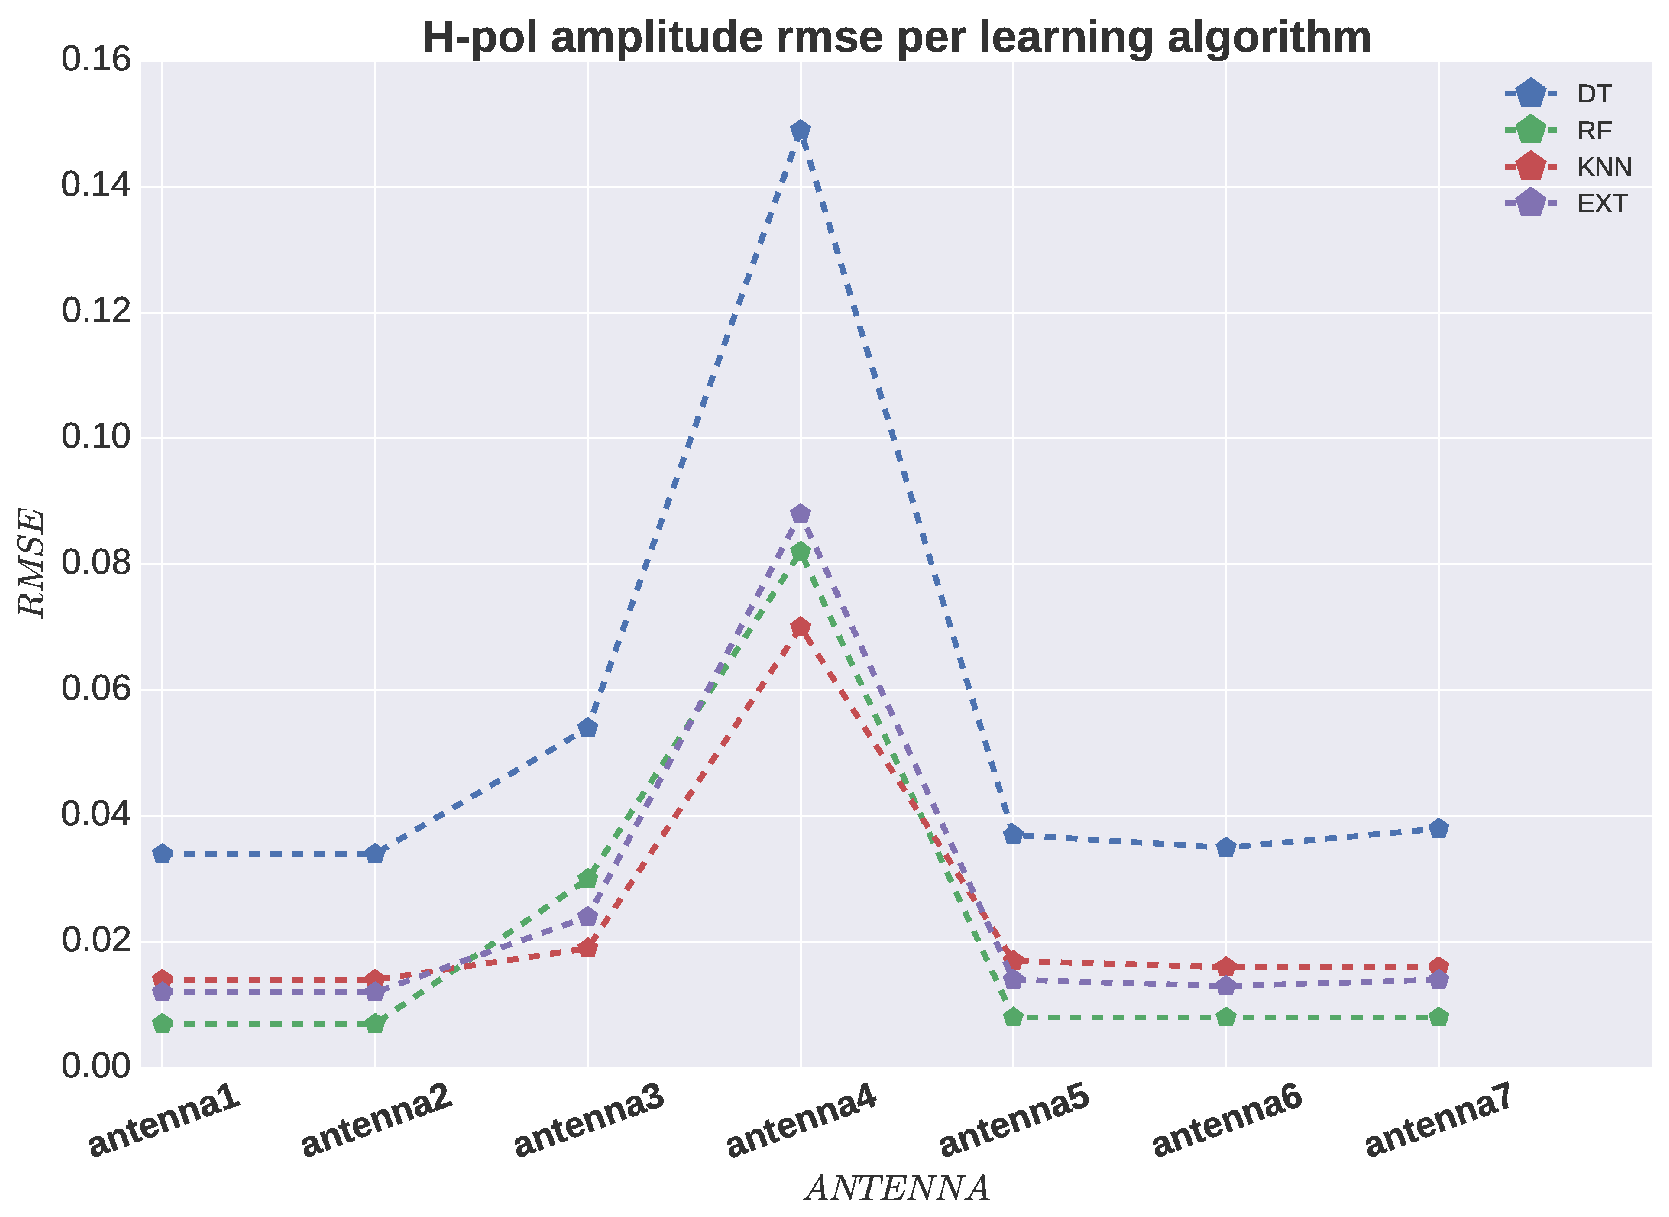
\includegraphics[width=0.6\textwidth]{images/Hpol-amp.eps}
    \caption{Root mean square error for each learning algorithm in predicting the h polarization amplitude gain solutions for each antenna. The blue, green, red and purple lines represent the different learning algorithms used in our experiment.}
  \label{amprm}
 \end{figure} 

From the plot in Figure \ref{amprm}, we observe that the random forest, K-nearest neighbour, and extremely randomized trees have quite learned to predict the h polarization amplitude gain solutions with an rms error accuracy of less than $0.02$, which is much better when compared to the phase prediction in Figure \ref{phrm}. Similar to h polarization phase prediction, we observe a large rms error variation on antenna 3h and 4h in all 4 models, with decision trees having large rms error scattering than the rest. From validation data sets, the Figures \ref{da1}, \ref{ka1}, \ref{ra1}, \ref{ea1} are showing the decision tree output prediction from all the observation tests, and we observe that the decision tree model cannot generalize well for different new observational sets, thereby producing flat amplitude. However, the remaining three models are predicting the gain amplitude solutions when fed with new observational data set. These models managed to learn the most critical part i.e, the sinusoidal variation of the gain amplitude solutions over time. Figures \ref{ra1}, \ref{ra2}, \ref{ra3}, \ref{ea1}, \ref{ea2}, \ref{ea3} are showing good amplitude predictions for all the validation sets. Since the target of our experiment is the calibrator PKS1613-586, which was considered a bright source and a good calibrator during KAT-7 commissioning. We therefore compare the h polarization amplitude experimental solutions with ones obtained from CASA through calibration of the validation data sets. We observe that the machine learning amplitude is lower than CASA with a factor of 33.33$\%$ for observation test-1 and 22.22 $\%$ for observation test-2, test-3. On the other hand, the K-nearest neighbor seems to have failed in observation test-1 and predicted approximately close to CASA for observation test-2 and test-3.

In Figure \ref{ra2} and \ref{ea2}, The model predicts a drop  of amplitude as a function time in the middle of the observation from from 0.12 to 0.09 level of CASA. This is a unique behaviour observed in observation test-2. This proves that the random forest and extremely randomized trees have learned to generalize and also can spot suspicious unexplained behaviour seen from environmental and pointing sensors that can not be seen when calibrating only through CASA.  
\section{V-polarization amplitude and phase}
\label{Vp}
\begin{figure}[H]
  \centering
    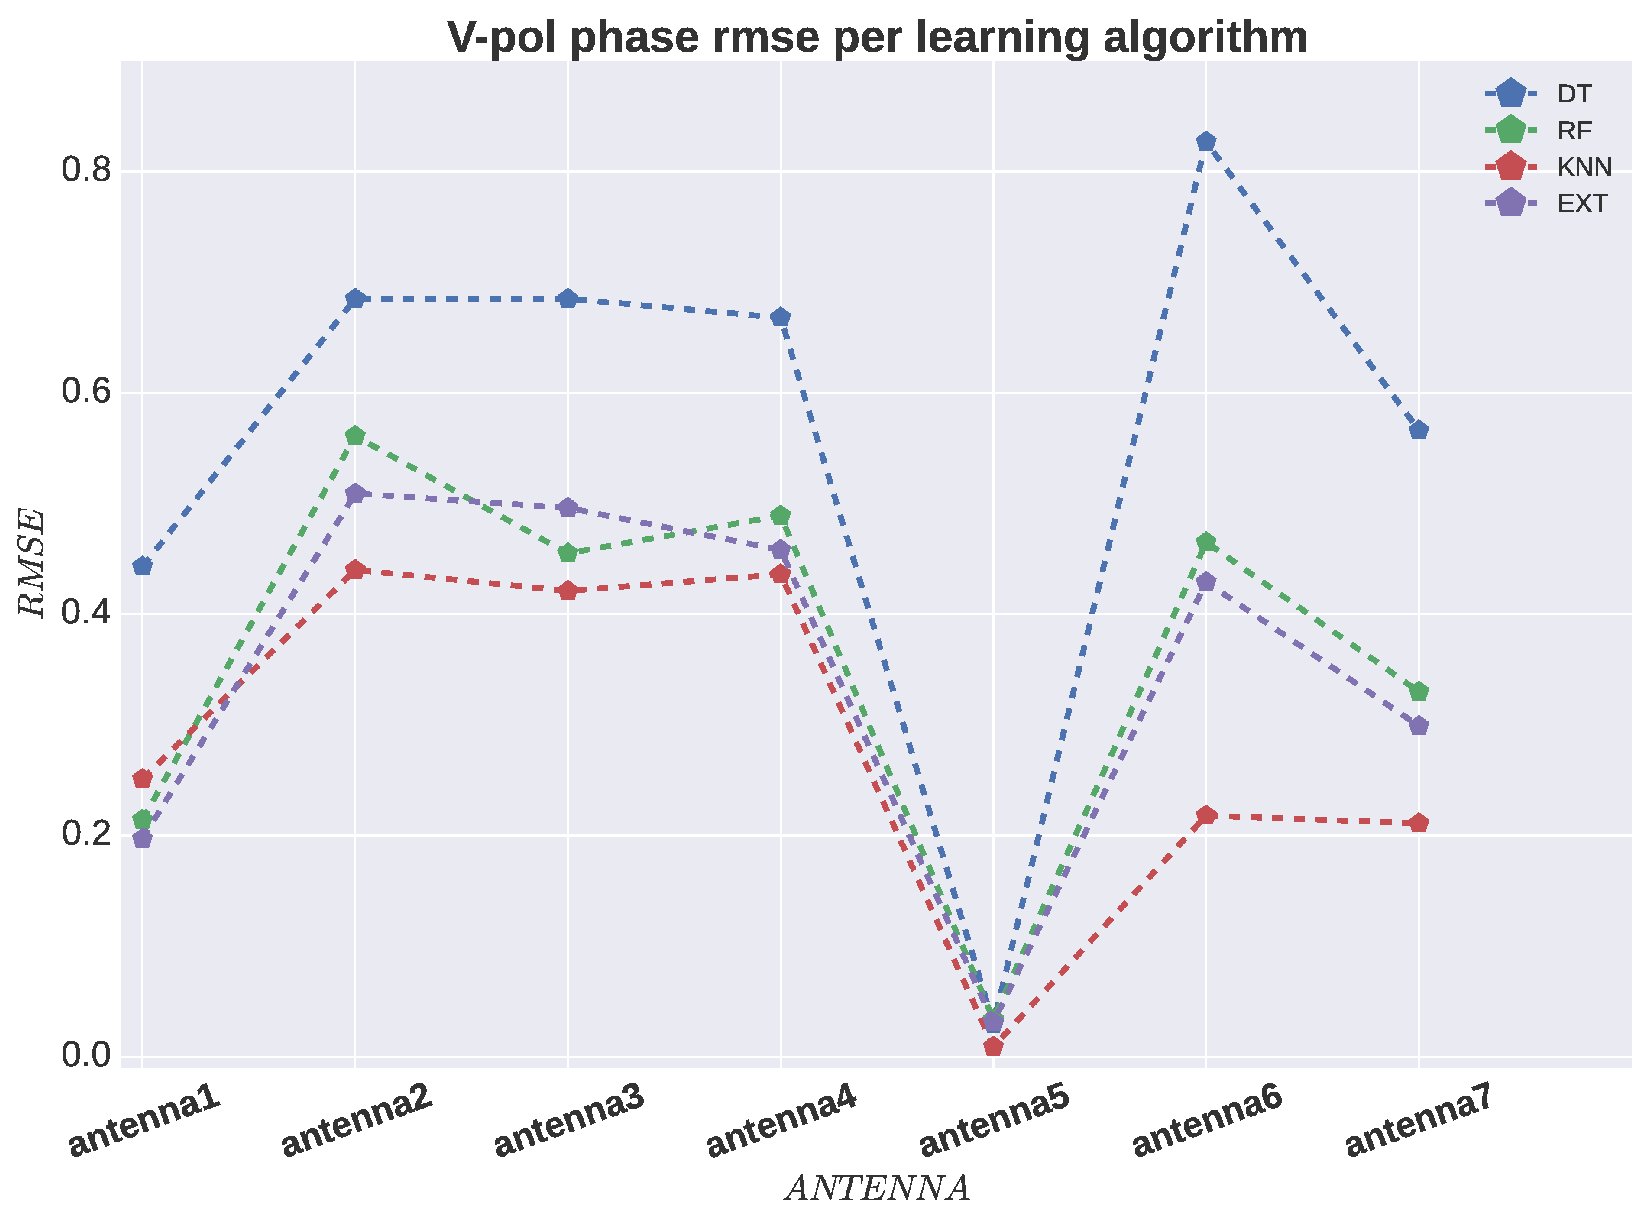
\includegraphics[width=0.6\textwidth]{images/Vpol-phase.eps}
    \caption{Root mean square error for each learning algorithm in predicting the v polarization phase gain solutions for each antenna. The blue, green, red and purple lines represent the different learning algorithms used in our experiment.}
  \label{phrmv}
 \end{figure}
The model behaviour for v polarization phase solutions experiment in Figure \ref{phrmv} is closely similar to Figure \ref{phrm} h polarization, except now there is large rms error variation on antenna 2 and 6 and 7, with random forest, K-nearest neighbors and the extremely randomized trees models showing much lower rms error accuracy score. When introducing the validation data sets for v polarization phase prediction, the random forest and extremely randomized tree in Figure \ref{obs6} and \ref{obs8} are fairly predicting stable v polarization phase solutions for observation test-2 and test-3.

In Figure \ref{phrm} and \ref{phrmv} The rms error increase from antenna 2,3,4 has an impact in the prediction of h and v polarization phase gain solution as shown in Figure \ref{obs6}, \ref{obs7}, \ref{obs8},\ref{obs10}, \ref{obs11}, \ref{obs12} for random forest, extremely randomized tree and K-nearest neighbor. We observe that solutions in antenna 2,3,4 are poorly predicted when compared to antenna 1,5,6 and 7. 

\begin{figure}[H]
  \centering
    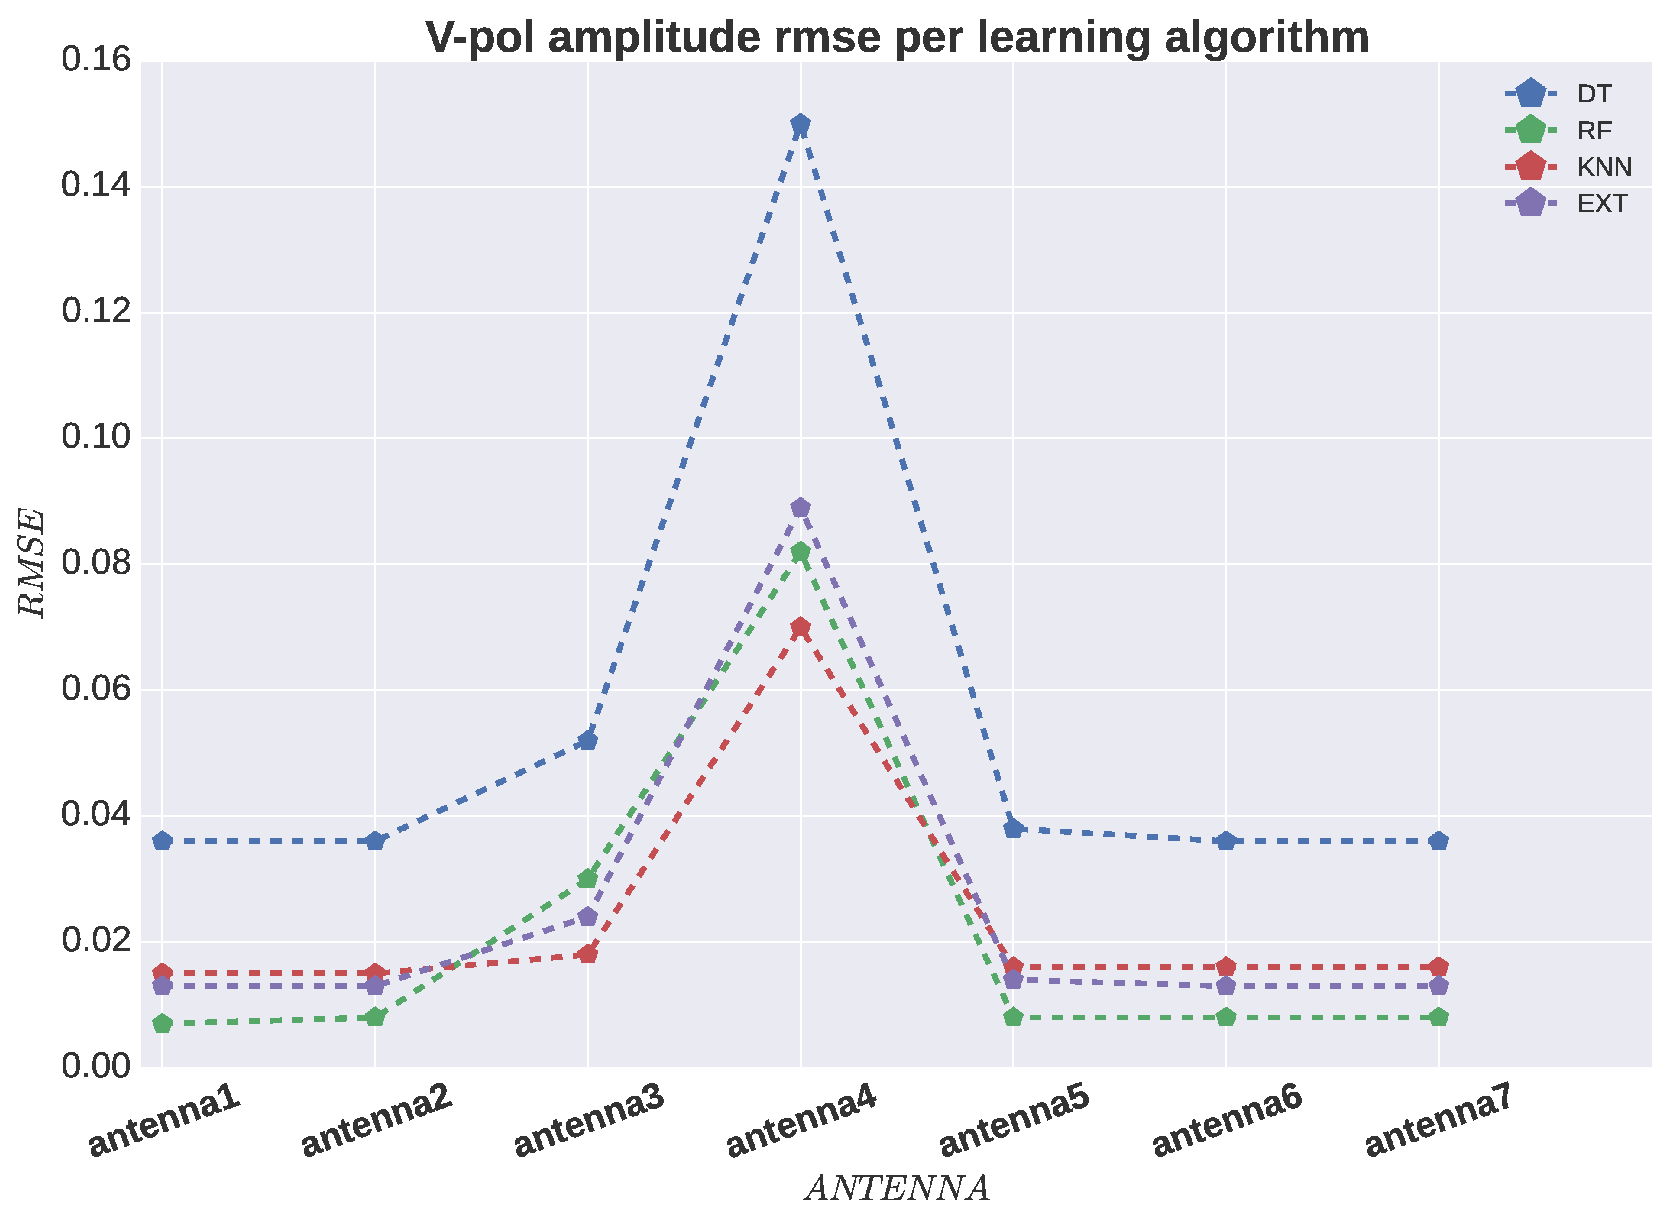
\includegraphics[width=0.6\textwidth]{images/Vpol-amp.eps}
    \caption{Root mean square error for each learning algorithm in predicting the v polarization amplitude gain solutions for each antenna. The blue, green, red and purple lines represent the different learning algorithms used in our experiment.}
  \label{amprmv}
 \end{figure} 

The v polarization rms error is not different from h polarization as shown in Figures \ref{amprm} and \ref{amprmv}, where the rms error in both polarization for all the antennas is measured and rated the same. We observe similar amplitude  difference as in h polarization when camparing with CASA solutions, i.e with a factor of 33.33$\%$ for observation test-1 and 22.22 $\%$ for observation test-2, test-3. In Figures \ref{amprm} and \ref{amprmv}, the h and v amplitude rms error increase from antenna 3 to the high pick in antenna 4 has an impact in predicting the amplitude gain solutions. i.e, In Figures \ref{ra1}, \ref{ka1}, \ref{ea1}, \ref{ra2}, \ref{ka2}, \ref{ea2}, \ref{ra3} ,\ref{ka3}, \ref{ea3} we observe poor predicted gain amplitude solutions for antenna 3 and 4 for observation test-1,2,3 in random forest, K-nearest neighbor and extremely randomised models.

From the analysis above, we therefore conclude that the random forest and extremely randomised trees are the better models in predicting the amplitude and phase gain solutions followed by the K-nearest neighbor. However, these models have strongly learned to predict the amplitude gain solutions than phase. This can be most likely due to the fact that the machine learning was trained on limited amount of data, and therefore can not fully predict on what the sky is doing since the phase is sensitive varies quickly over time as a function of antenna based(ground) and sky based effects.  As for amplitude, most of its effect are instrument based and the environment around it, hence it is doing better than phase prediction in our experiment. Some of the limitations of our experiment may be due to training being done on time based calibration solutions and not frequency (bandpass). 

When comparing the bias/variance of the tree based methods, we observe that algorithm randomization increases bias and variance of individual trees, but  may decrease their variance with respect to the learning sample. The part of the variance due to randomization can be cancelled out by averaging over a
sufficiently large ensemble of trees. overall, the bias/variance tradeoff is different in regression than in classification problems;
in particular, classification problems can tolerate high levels of bias of class probability estimates without yielding high classification error rates \citep{geurts2006extremely}. 

During model training, Random Forests pre-sort the learning sample before growing all trees to avoid having to re-sort it each time a node is split. This pre-sorting reduced the average computing times of this method. However, the implementation of Extremely randomized trees, on the other hand, does not use pre-sorting, which is a further advantage in the case of very large problems, where it may not be possible to keep in memory a sorted copy of the learning sample for each candidate feature. Since pre-sorting requires on the order of $nN\log N$ operations, it makes the
computational complexity of Random Forests depend linearly on the number of features. Hence, for very large numbers of attributes the computational advantage of Extra-Trees is even higher \citep{geurts2006extremely}.


\section{Appendix}
\subsection{Decision tree H\&V accuracy scores}

\begin{table}[H]
\label{T:equipos}
\begin{center}
\scalebox{0.55}{
\begin{tabular}{| c | c | c | c | c |}
\hline
Antenna & \multicolumn{4}{ c |}{\textbf{Decision tree Phase}}  \\ 
\cline{2-5}
&Rmse & Rmae & R2score & Explained $\sigma^2$\\
\hline

Ant1-H & 0.443 & 0.411 & 0.922    & 0.923     \\
Ant2-H &0.685 & 0.471 & 0.869    & 0.87      \\
Ant3-H &0.685 & 0.52  & 0.861    & 0.861     \\
Ant4-H &0.668 & 0.511 & 0.816    & 0.817     \\
Ant5-H &0.03  & 0.061 & 0.643    & 0.643     \\
Ant6-H &0.827 & 0.54  & 0.784    & 0.784     \\
Ant7-H &0.566 & 0.434 & 0.914    & 0.914     \\
Ant1-V &0.381 & 0.387 & 0.957    & 0.957     \\
Ant2-V &0.394 & 0.378 & 0.956    & 0.956     \\
Ant3-V &0.716 & 0.519 & 0.839    & 0.839     \\
Ant4-V &0.513 & 0.451 & 0.92     & 0.92      \\
Ant5-V &0.029 & 0.055 & 0.571    & 0.572     \\
Ant6-V &0.455 & 0.401 & 0.943    & 0.943     \\
Ant7-V &0.457 & 0.397 & 0.913    & 0.914     \\
 \hline
 & \multicolumn{4}{ c |}{\textbf{Decision tree Amplitude}}  \\ 
\cline{1-5}
\hline


Ant1-H&0.034 & 0.106 & 0.824    & 0.824     \\
Ant2-H&0.034 & 0.105 & 0.833    & 0.833     \\
Ant3-H&0.054 & 0.145 & 0.707    & 0.709     \\
Ant4-H&0.149 & 0.206 & 0.46     & 0.462     \\
Ant5-H&0.037 & 0.11  & 0.83     & 0.83      \\
Ant6-H&0.035 & 0.107 & 0.83     & 0.831     \\
Ant7-H&0.038 & 0.11  & 0.828    & 0.828     \\
Ant1-V&0.036 & 0.108 & 0.825    & 0.825     \\
Ant2-V&0.036 & 0.11  & 0.822    & 0.822     \\
Ant3-V&0.052 & 0.145 & 0.695    & 0.697     \\
Ant4-V&0.15  & 0.207 & 0.46     & 0.462     \\
Ant5-V&0.038 & 0.111 & 0.828    & 0.828     \\
Ant6-V&0.036 & 0.107 & 0.826    & 0.826     \\
Ant7-V&0.036 & 0.107 & 0.825    & 0.825     \\
\hline
\end{tabular}}
\end{center}
\end{table}

\subsection{Random forest H\& V accuracy scores}

\begin{table}[H]
\begin{center}
\scalebox{0.55}{
\begin{tabular}{| c | c | c | c | c |}
\hline
Antenna & \multicolumn{4}{ c |}{\textbf{Random forest Phase}}  \\ 
\cline{2-5}
& Rmse & Rmae & R2score & Explained $\sigma^2$\\
\hline

Ant1-H&0.214 & 0.326 & 0.982    & 0.982     \\
Ant2-H&0.561 & 0.459 & 0.912    & 0.912     \\
Ant3-H&0.455 & 0.439 & 0.939    & 0.94      \\
Ant4-H&0.489 & 0.418 & 0.901    & 0.902     \\
Ant5-H&0.034 & 0.07  & 0.564    & 0.564     \\
Ant6-H&0.465 & 0.417 & 0.931    & 0.932     \\
Ant7-H&0.33  & 0.369 & 0.971    & 0.971     \\
Ant1-V&0.216 & 0.318 & 0.986    & 0.986     \\
Ant2-V&0.283 & 0.355 & 0.977    & 0.977     \\
Ant3-V&0.447 & 0.43  & 0.937    & 0.937     \\
Ant4-V&0.365 & 0.416 & 0.959    & 0.959     \\
Ant5-V&0.031 & 0.062 & 0.516    & 0.516     \\
Ant6-V&0.267 & 0.354 & 0.981    & 0.981     \\
Ant7-V&0.198 & 0.299 & 0.984    & 0.984     \\ 
  \hline
 & \multicolumn{4}{ c |}{\textbf{Random forest Amplitude}}  \\ 
\cline{1-5}
\hline

Ant1-H&0.007 & 0.063 & 0.992    & 0.992     \\
Ant2-H&0.007 & 0.064 & 0.992    & 0.992     \\
Ant3-H&0.03  & 0.113 & 0.911    & 0.914     \\
Ant4-H&0.082 & 0.17  & 0.838    & 0.838     \\
Ant5-H&0.008 & 0.065 & 0.993    & 0.993     \\
Ant6-H&0.008 & 0.063 & 0.992    & 0.992     \\
Ant7-H&0.008 & 0.064 & 0.992    & 0.992     \\
Ant1-V&0.007 & 0.063 & 0.992    & 0.992     \\
Ant2-V&0.008 & 0.066 & 0.991    & 0.991     \\
Ant3-V&0.03  & 0.113 & 0.9      & 0.903     \\
Ant4-V&0.082 & 0.171 & 0.837    & 0.837     \\
Ant5-v&0.008 & 0.066 & 0.993    & 0.993     \\
Ant6-V&0.008 & 0.063 & 0.992    & 0.992     \\
Ant7-V&0.008 & 0.062 & 0.992    & 0.992     \\ 
 \hline
\end{tabular}}
\end{center}
\end{table}

\subsection{K-Nearest Neighbor H\&V accuracy scores}

\begin{table}[H]
\label{T:equipos}
\begin{center}
\scalebox{0.55}{
\begin{tabular}{| c | c | c | c | c |}
\hline
\textbf{Antenna} & \multicolumn{4}{ c |}{\textbf{KNN Phase}}  \\ 
\cline{2-5}
& Rmse & Rmae & R2score & Explained $\sigma^2$\\
\hline

Ant1-H &0.251 & 0.24  & 0.975    & 0.975     \\
Ant2-H &0.44  & 0.317 & 0.946    & 0.946     \\
Ant3-H &0.421 & 0.296 & 0.948    & 0.948     \\
Ant4-H &0.436 & 0.321 & 0.922    & 0.922     \\
Ant5-H &0.009 & 0.033 & 0.967    & 0.967     \\
Ant6-H &0.218 & 0.22  & 0.985    & 0.985     \\
Ant7-H &0.211 & 0.206 & 0.988    & 0.988     \\
Ant1-V &0.199 & 0.21  & 0.988    & 0.988     \\
Ant2-V &0.281 & 0.251 & 0.978    & 0.978     \\
Ant3-V &0.207 & 0.215 & 0.987    & 0.987     \\
Ant4-V &0.216 & 0.248 & 0.986    & 0.986     \\
Ant5-V &0.006 & 0.027 & 0.98     & 0.98      \\
Ant6-V &0.306 & 0.25  & 0.974    & 0.974     \\
Ant7-V &0.194 & 0.189 & 0.984    & 0.985     \\ 
 \hline
 & \multicolumn{4}{ c |}{\textbf{KNN Amplitude}}  \\ 
\cline{1-5}
\hline


Ant1-H&0.014 & 0.05  & 0.967    & 0.967     \\
Ant2-H&0.014 & 0.048 & 0.972    & 0.973     \\
Ant3-H&0.019 & 0.063 & 0.962    & 0.962     \\
Ant4-H&0.07  & 0.107 & 0.883    & 0.883     \\
Ant5-H&0.017 & 0.053 & 0.966    & 0.966     \\
Ant6-H&0.016 & 0.053 & 0.965    & 0.965     \\
Ant7-H&0.016 & 0.052 & 0.968    & 0.968     \\
Ant1-V&0.015 & 0.05  & 0.969    & 0.969     \\
Ant2-V&0.015 & 0.05  & 0.968    & 0.968     \\
Ant3-V&0.018 & 0.062 & 0.963    & 0.963     \\
Ant4-V&0.07  & 0.108 & 0.882    & 0.882     \\
Ant5-V&0.016 & 0.052 & 0.968    & 0.968     \\
Ant6-V&0.016 & 0.052 & 0.965    & 0.965     \\
Ant7-V&0.016 & 0.05  & 0.967    & 0.968     \\ 
 \hline

\end{tabular}}
\end{center}
\end{table}


\subsection{Extremely randomised tree H\&V accuracy scores}

\begin{table}[H]
\label{T:equipos}
\begin{center}
\scalebox{0.55}{
\begin{tabular}{| c | c | c | c | c |}
\hline
Antenna & \multicolumn{4}{ c |}{\textbf{Extremely randomized Phase}}  \\ 
\cline{2-5}
& Rmse & Rmae &R2score & Explained  $\sigma^2$\\
\hline

Ant1-H&0.197 & 0.305 & 0.985    & 0.985     \\
Ant2-H&0.509 & 0.439 & 0.928    & 0.928     \\
Ant3-H&0.496 & 0.42  & 0.927    & 0.928     \\
Ant4-H&0.458 & 0.409 & 0.914    & 0.914     \\
Ant5-H&0.031 & 0.062 & 0.63     & 0.63      \\
Ant6-H&0.429 & 0.391 & 0.942    & 0.942     \\
Ant7-H&0.299 & 0.348 & 0.976    & 0.976     \\
Ant1-V&0.18  & 0.295 & 0.99     & 0.99      \\
Ant2-V&0.245 & 0.331 & 0.983    & 0.983     \\
Ant3-V&0.385 & 0.384 & 0.954    & 0.954     \\
Ant4-V&0.314 & 0.383 & 0.97     & 0.97      \\
Ant5-V&0.028 & 0.056 & 0.587    & 0.588     \\
Ant6-V&0.217 & 0.332 & 0.987    & 0.987     \\
Ant7-V&0.178 & 0.288 & 0.987    & 0.987    \\
  \hline
 & \multicolumn{4}{ c |}{\textbf{Extremely randomized tree  Amplitude}}  \\ 
\cline{1-5}
\hline

Ant1-H&0.012 & 0.068 & 0.976    & 0.976     \\
Ant2-H&0.012 & 0.068 & 0.978    & 0.979     \\
Ant3-H&0.024 & 0.1   & 0.942    & 0.943     \\
Ant4-H&0.088 & 0.161 & 0.811    & 0.811     \\
Ant5-H&0.014 & 0.07  & 0.976    & 0.976     \\
Ant6-H&0.013 & 0.069 & 0.976    & 0.976     \\
Ant7-H&0.014 & 0.071 & 0.977    & 0.977     \\
Ant1-V&0.013 & 0.069 & 0.977    & 0.977     \\
Ant2-V&0.013 & 0.07  & 0.976    & 0.976     \\
Ant3-V&0.024 & 0.1   & 0.937    & 0.938     \\
Ant4-V&0.089 & 0.161 & 0.81     & 0.81      \\
Ant5-V&0.014 & 0.071 & 0.977    & 0.977     \\
Ant6-V&0.013 & 0.069 & 0.976    & 0.976     \\
Ant7-V&0.013 & 0.069 & 0.976    & 0.976    \\ 
 \hline
\end{tabular}}
\end{center}
\end{table}

%An average research project may contain five chapters, but I didn't plan my work properly
%and then ran out of time. I spent too much time positioning my figures and worrying
%about my preferred typographic style, rather than just using what was provided.
%I wasted days bolding section headings and using double slash line endings, and 
%had to remove them all again. I spent sleepless nights configuring manually numbered lists
%to use the \LaTeX\ environments because I didn't use them from the start or understand
%how to search and replace easily with texmaker.
%
%Everyone has to take some shortcuts
%at some point to meet deadlines. Time did not allow to test model 
%B as well. So I'll skip right ahead and put that under my Future Work section.
%
%
%\section{This is a section} 
%
%Some research projects may have 3, 5 or 6 chapters. This is just an example. 
%More importantly, do you have at close to 30 pages?  
%Luck has nothing to do with it. Use the techniques suggested for
%writing your research project.
%
%Now you're demonstrating pure talent and newly acquired skills. 
%Perhaps some persistence. Definitely some inspiration. What was that about perspiration? 
%Some team work helps, so every now and then why not browse your friends' research project and provide
%some constructive feedback?
%
%\subsection{Subsubsections are disabled}
%
%Vivamus faucibus arcu ut cursus maximus. Aenean ac aliquet nulla. Duis efficitur varius malesuada. Etiam finibus risus et condimentum commodo. Mauris interdum ligula ut lacinia blandit. Curabitur commodo, mauris vel porttitor semper, ante risus pellentesque ipsum, non commodo sapien massa quis tortor. Vestibulum ante ipsum primis in faucibus orci luctus et ultrices posuere cubilia Curae; Phasellus ac massa commodo purus placerat pharetra id ut ex. Nam malesuada, turpis vel iaculis sodales, nisl ante fringilla tellus, et efficitur nisl felis at ligula. 
